\section*{Overview - Master's thesis }
The first task of the Master's thesis is to do a sanity check with the paper \cite{Bruna2012}. 
\begin{figure}[h!]
	\centering
	\hfill
	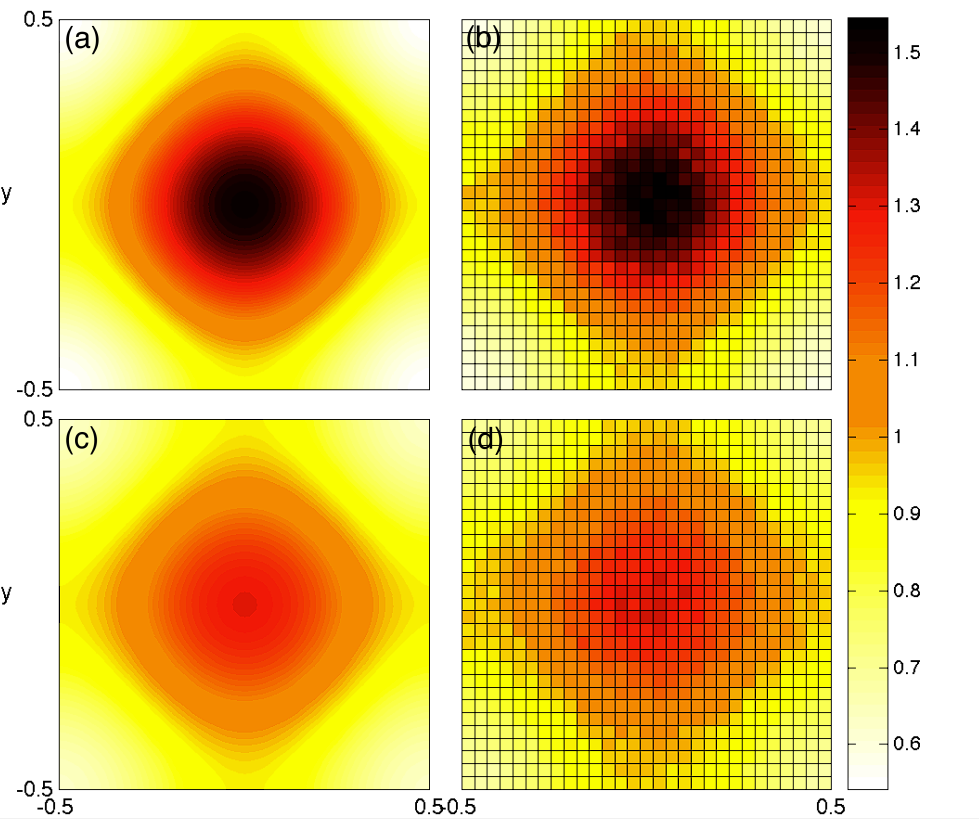
\includegraphics[width=\textwidth]{sanity-check/bruna12_theOriginal.png}
\end{figure}
Until now, we made 2 bigger simulations. We neglected the interior angle force, because it caused stability problems. 

\newpage
\subsection*{First big simulation}
Here is our most recent simulation parameters:
\begin{itemize}
    \item 16 cells are spawned at a fixes 4x4 initial state 
    \item 40 wall points per cell 
    \item Diffusitivity constant $D=5.0$
    \item bachelor scalings, but wihtout interior angle force for better stability
    \item $time interval = [0, 100]$
    \item $time step size = 2^{-8}$
    \item used bachelor overlap 
    \item 300 simulations ran 
    \item $grid = [-5,5]^2$ with discretisation step size $\delta x = 0.25$
\end{itemize}

% FIGURE OF FIRST BIG SIMULATION
\begin{figure}[h!]
	\centering
	\begin{subfigure}{0.4\textwidth}
		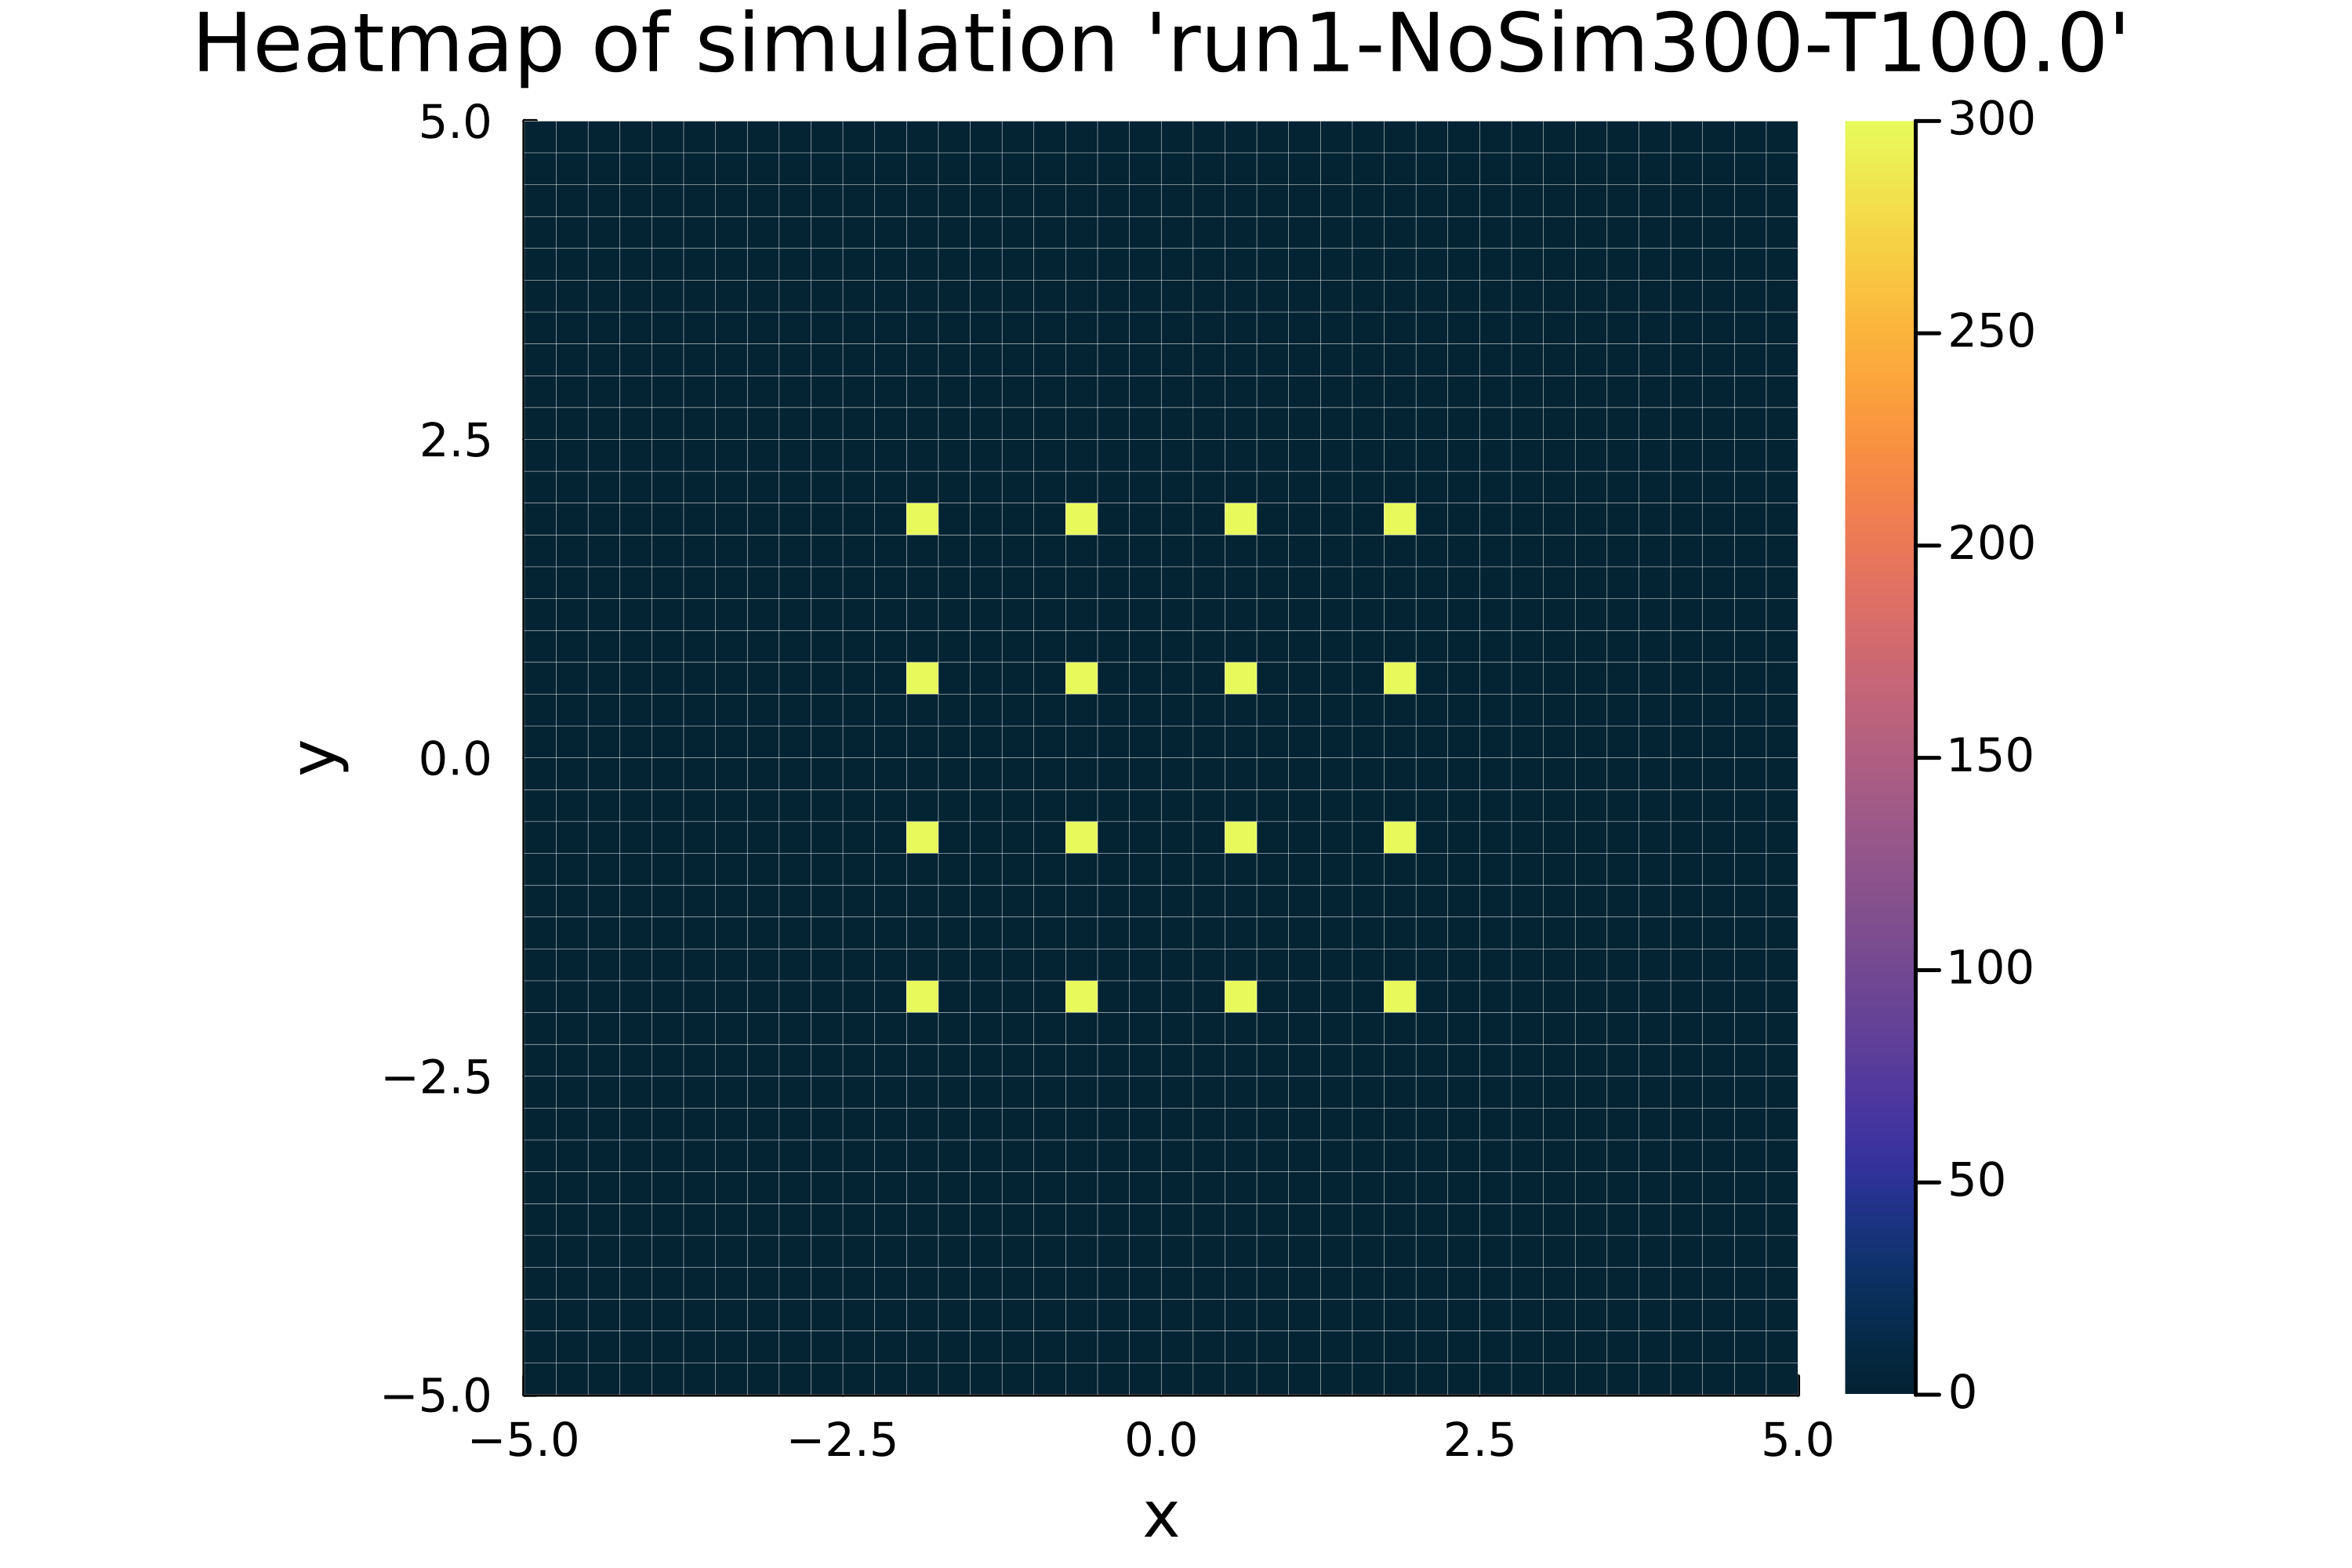
\includegraphics[width=\textwidth]{sanity-check/Heatmap-run1-NoSim300-T100.0/heatmaps/heatmap-run1-NoSim300-T100.0-sampleTime0001.png}
	\end{subfigure}
	\hfill
	\begin{subfigure}{0.4\textwidth}
		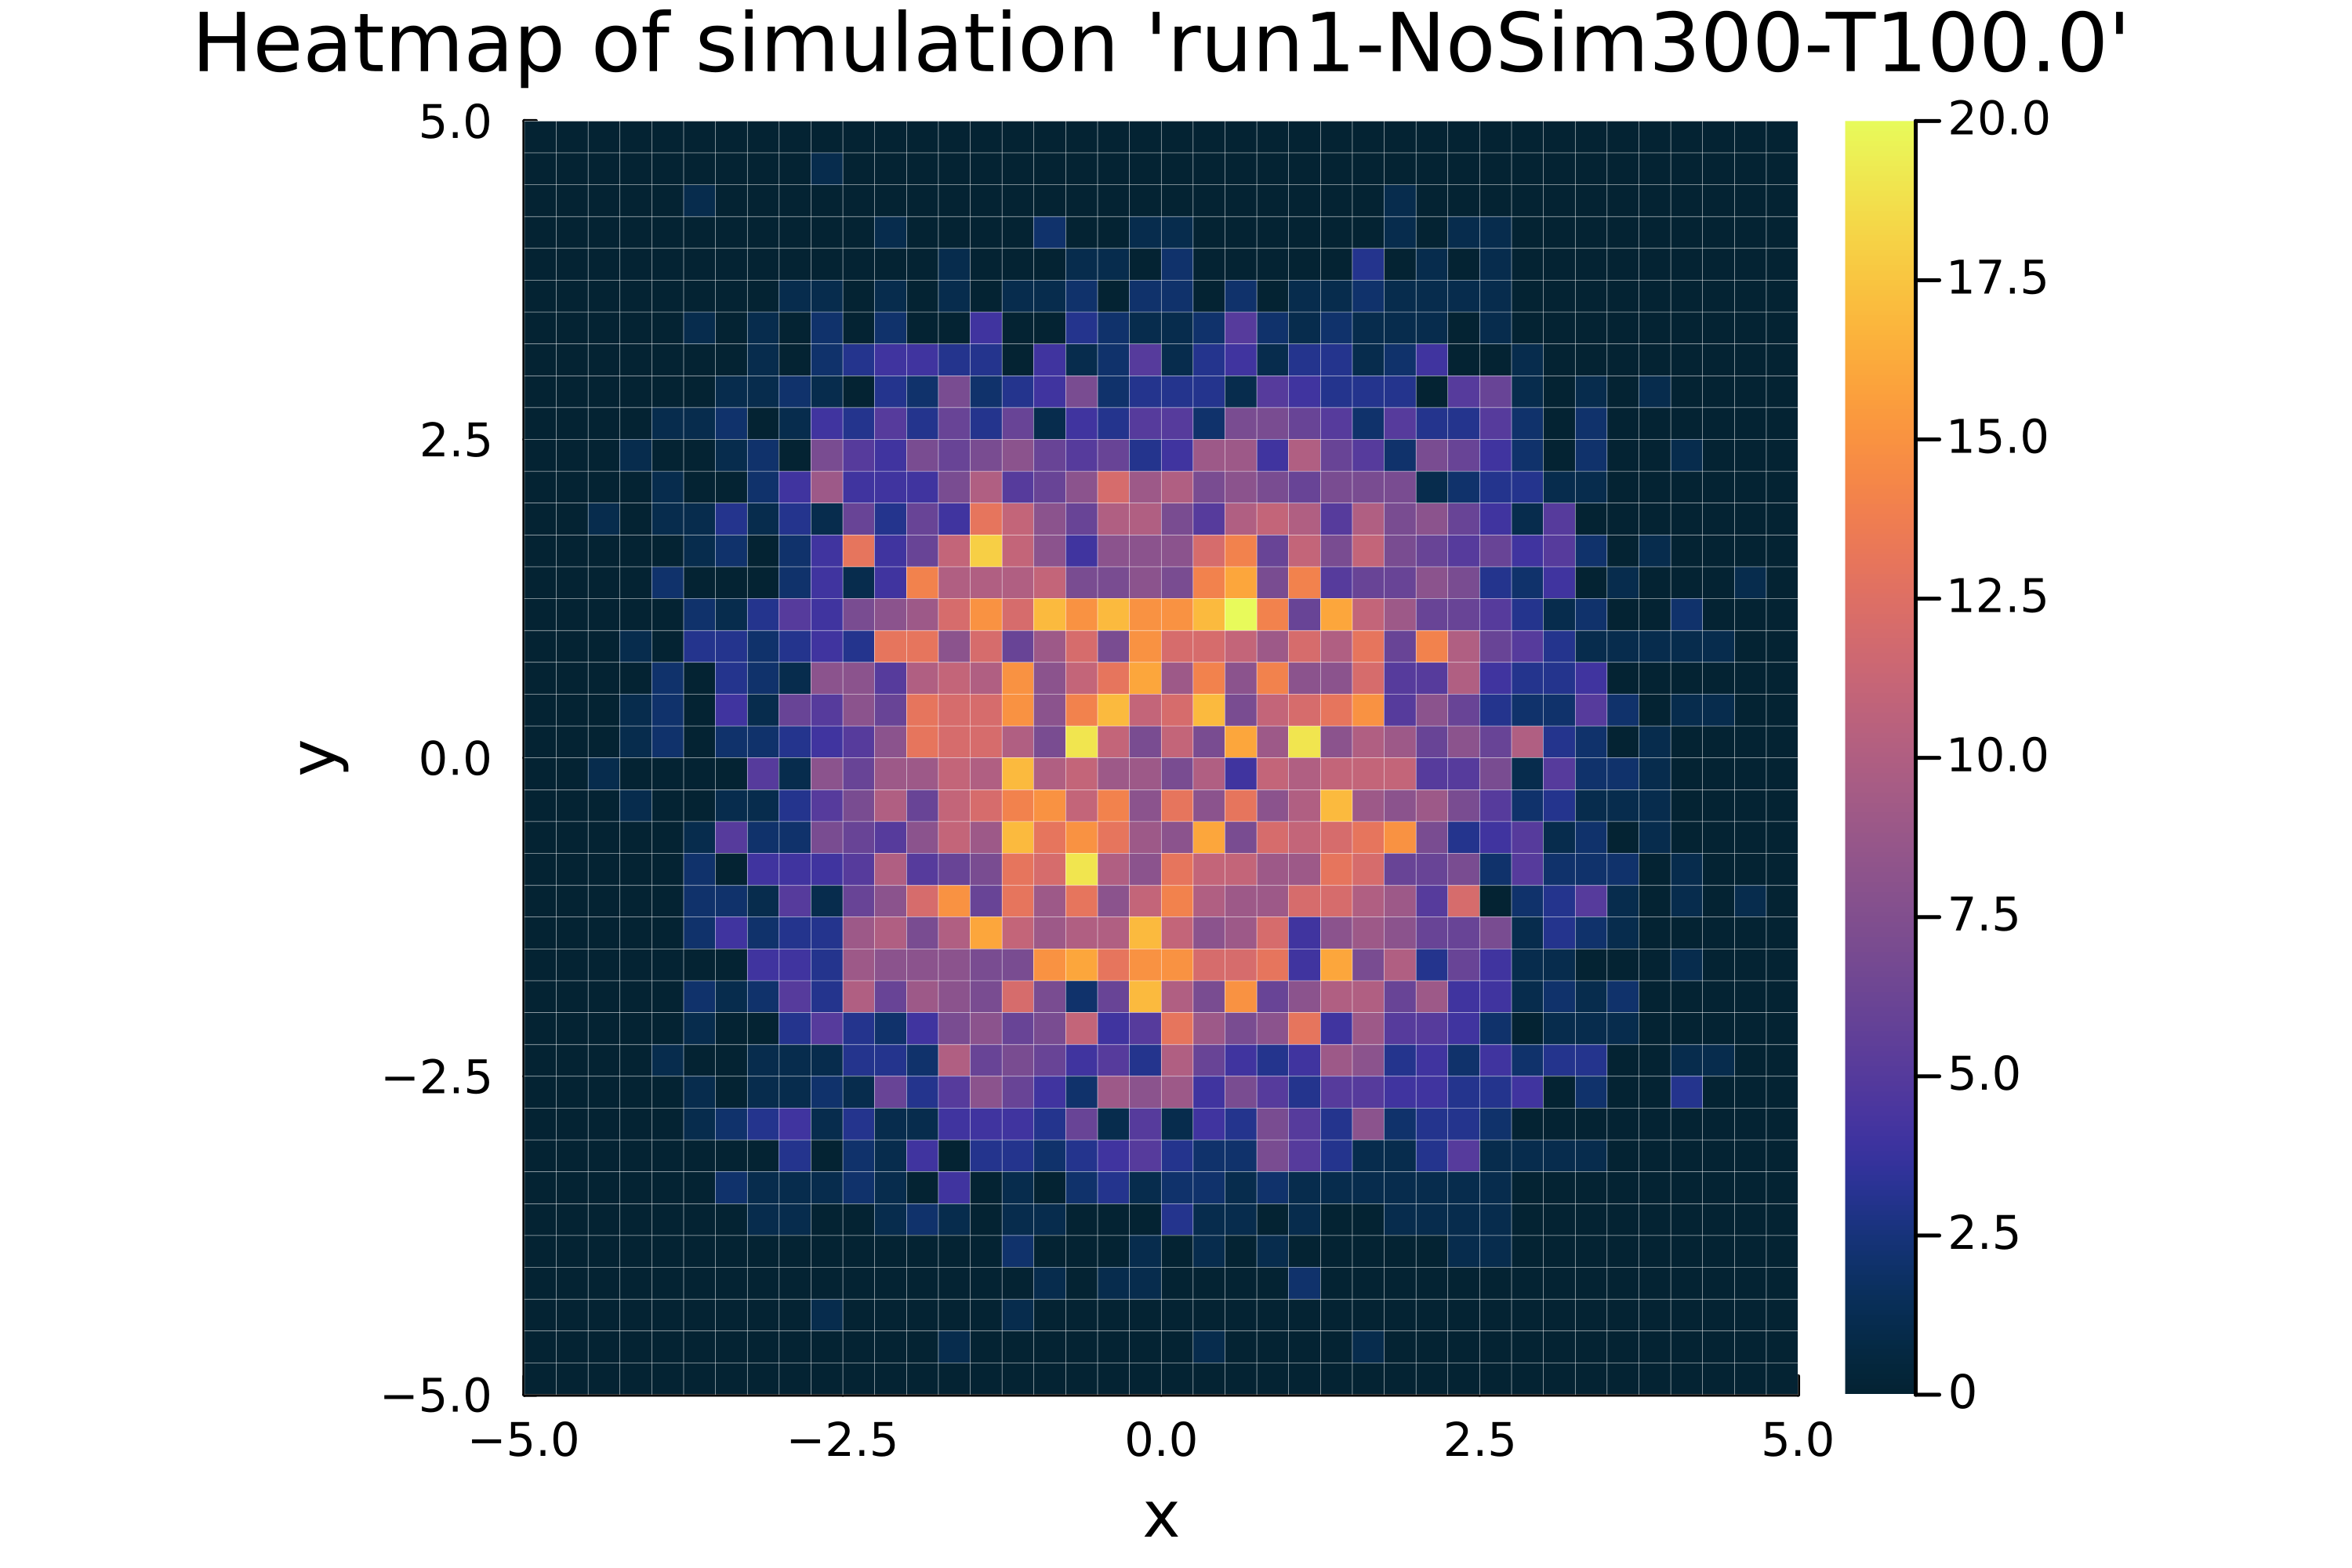
\includegraphics[width=\textwidth]{sanity-check/Heatmap-run1-NoSim300-T100.0/heatmaps/heatmap-run1-NoSim300-T100.0-sampleTime5000.png}
	\end{subfigure}
	\hfill
	\begin{subfigure}{0.4\textwidth}
		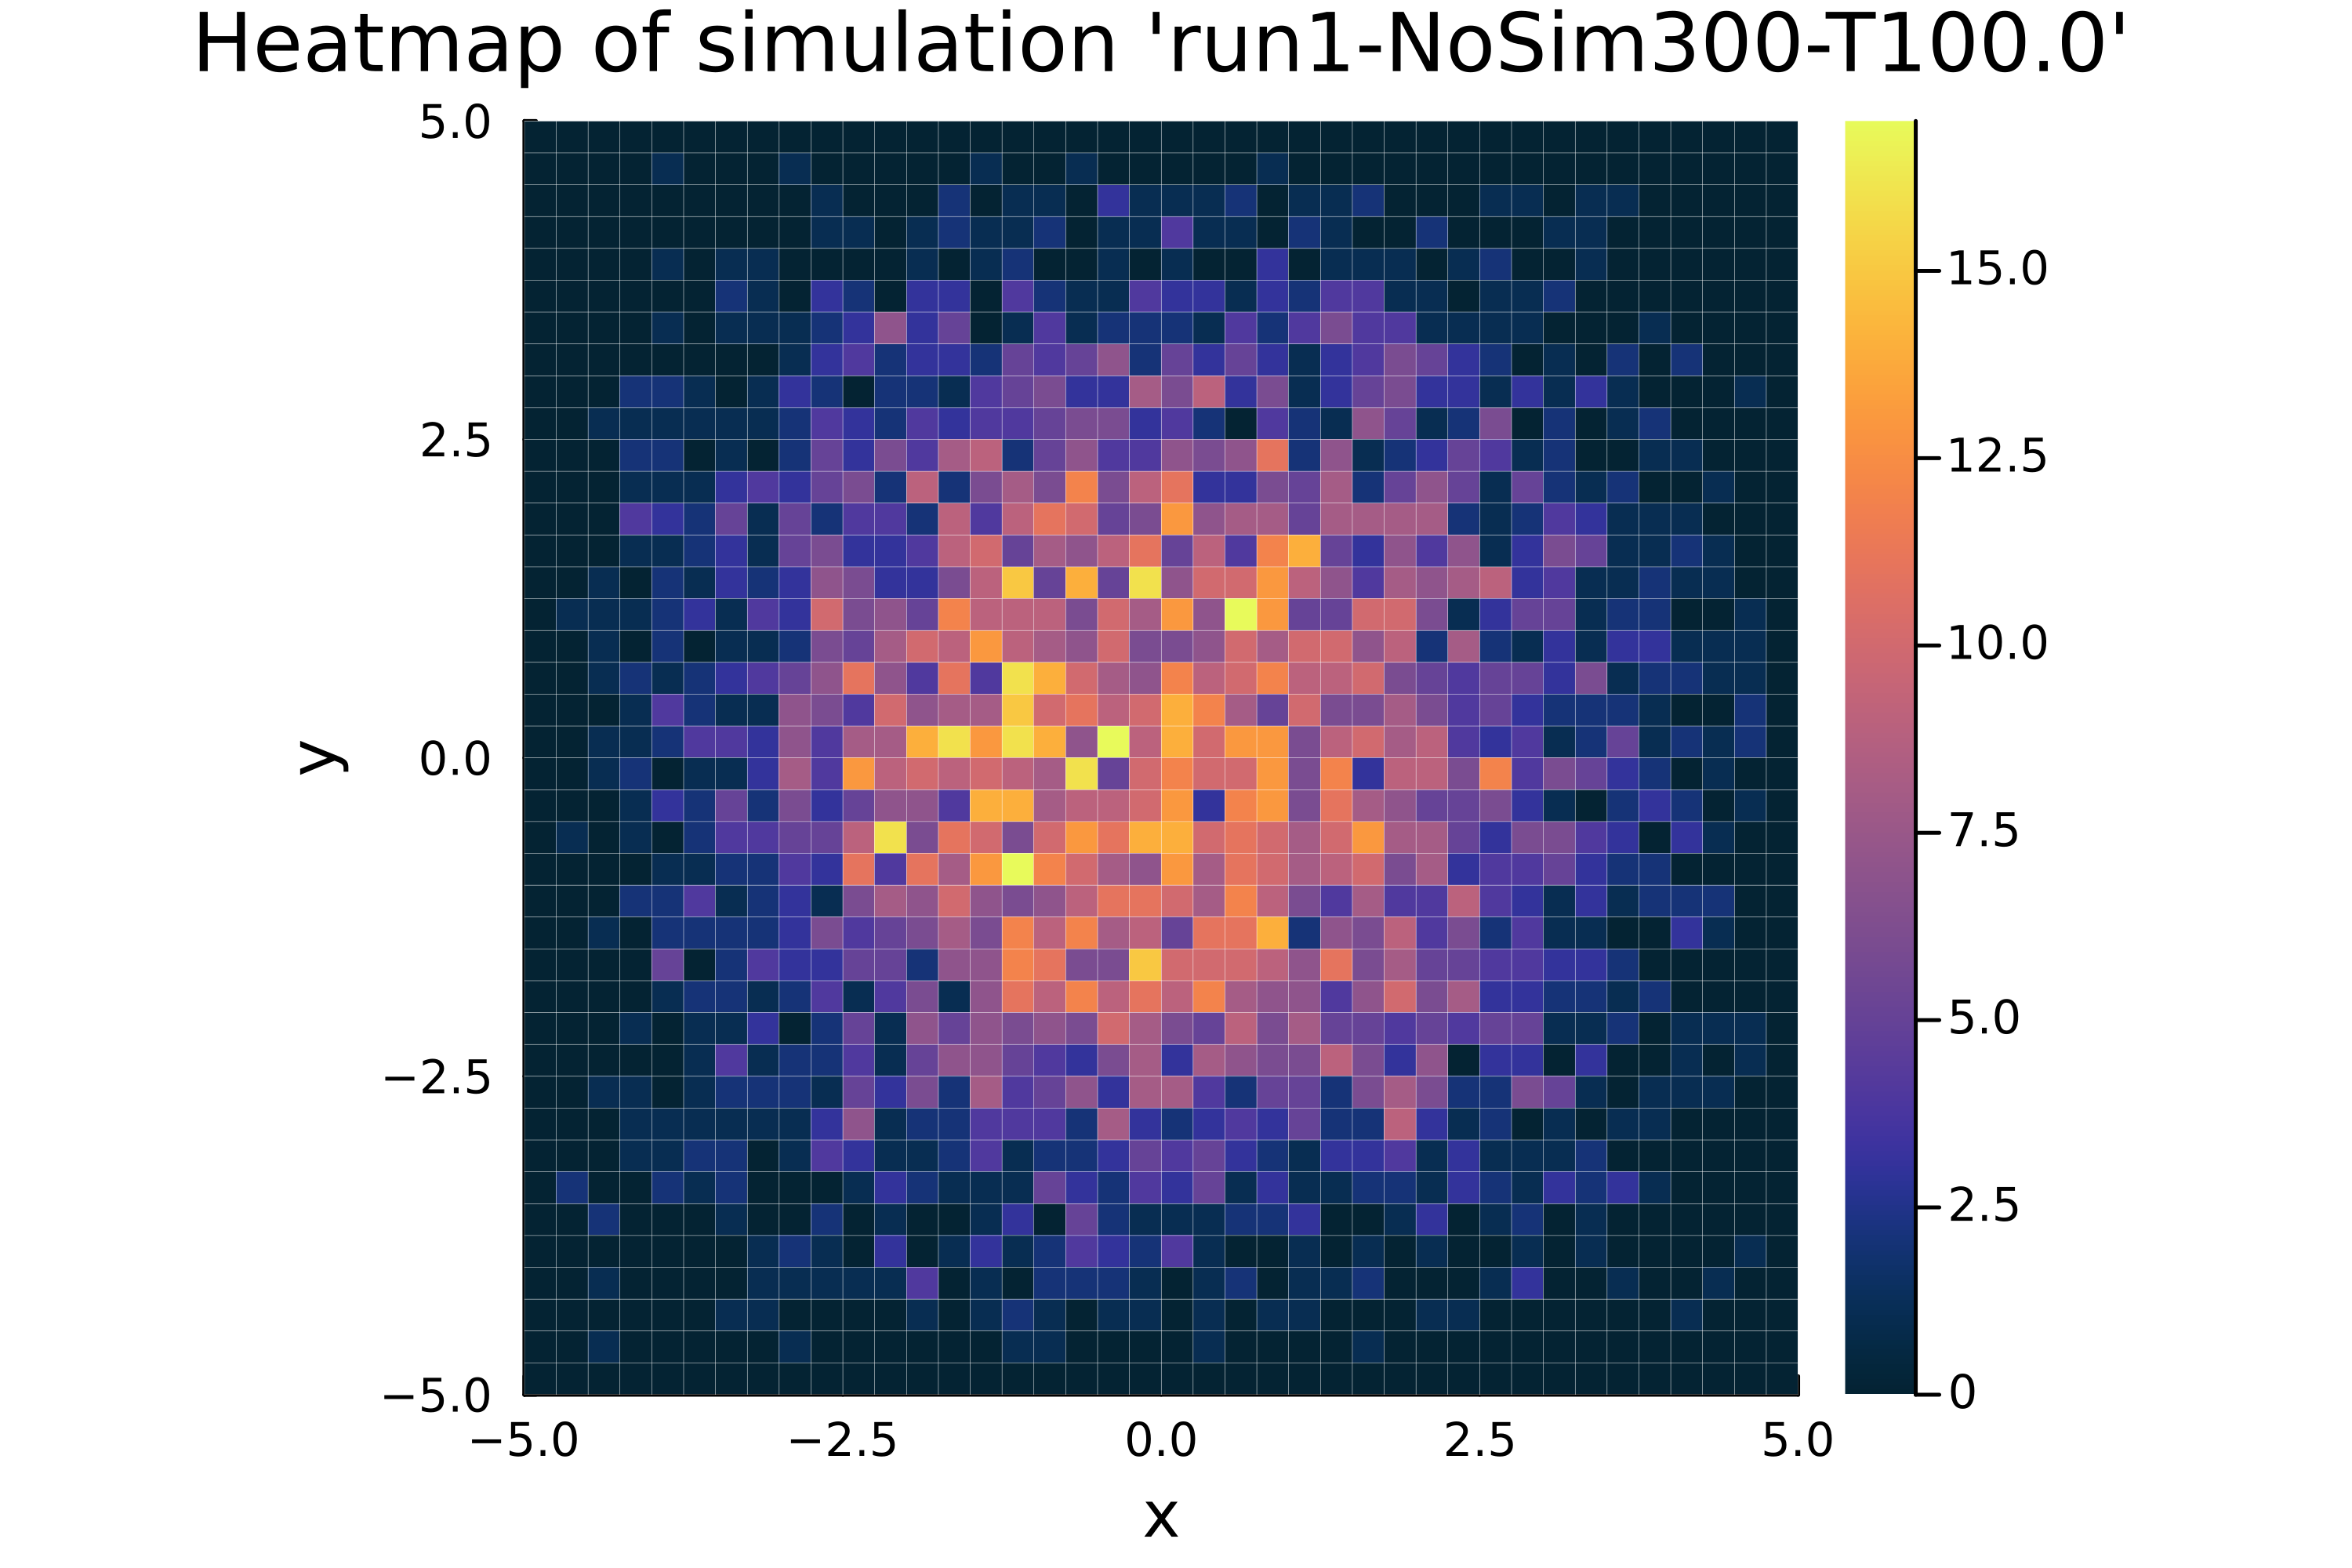
\includegraphics[width=\textwidth]{sanity-check/Heatmap-run1-NoSim300-T100.0/heatmaps/heatmap-run1-NoSim300-T100.0-sampleTime10000.png}
	\end{subfigure}\hfill
	\begin{subfigure}{0.4\textwidth}
		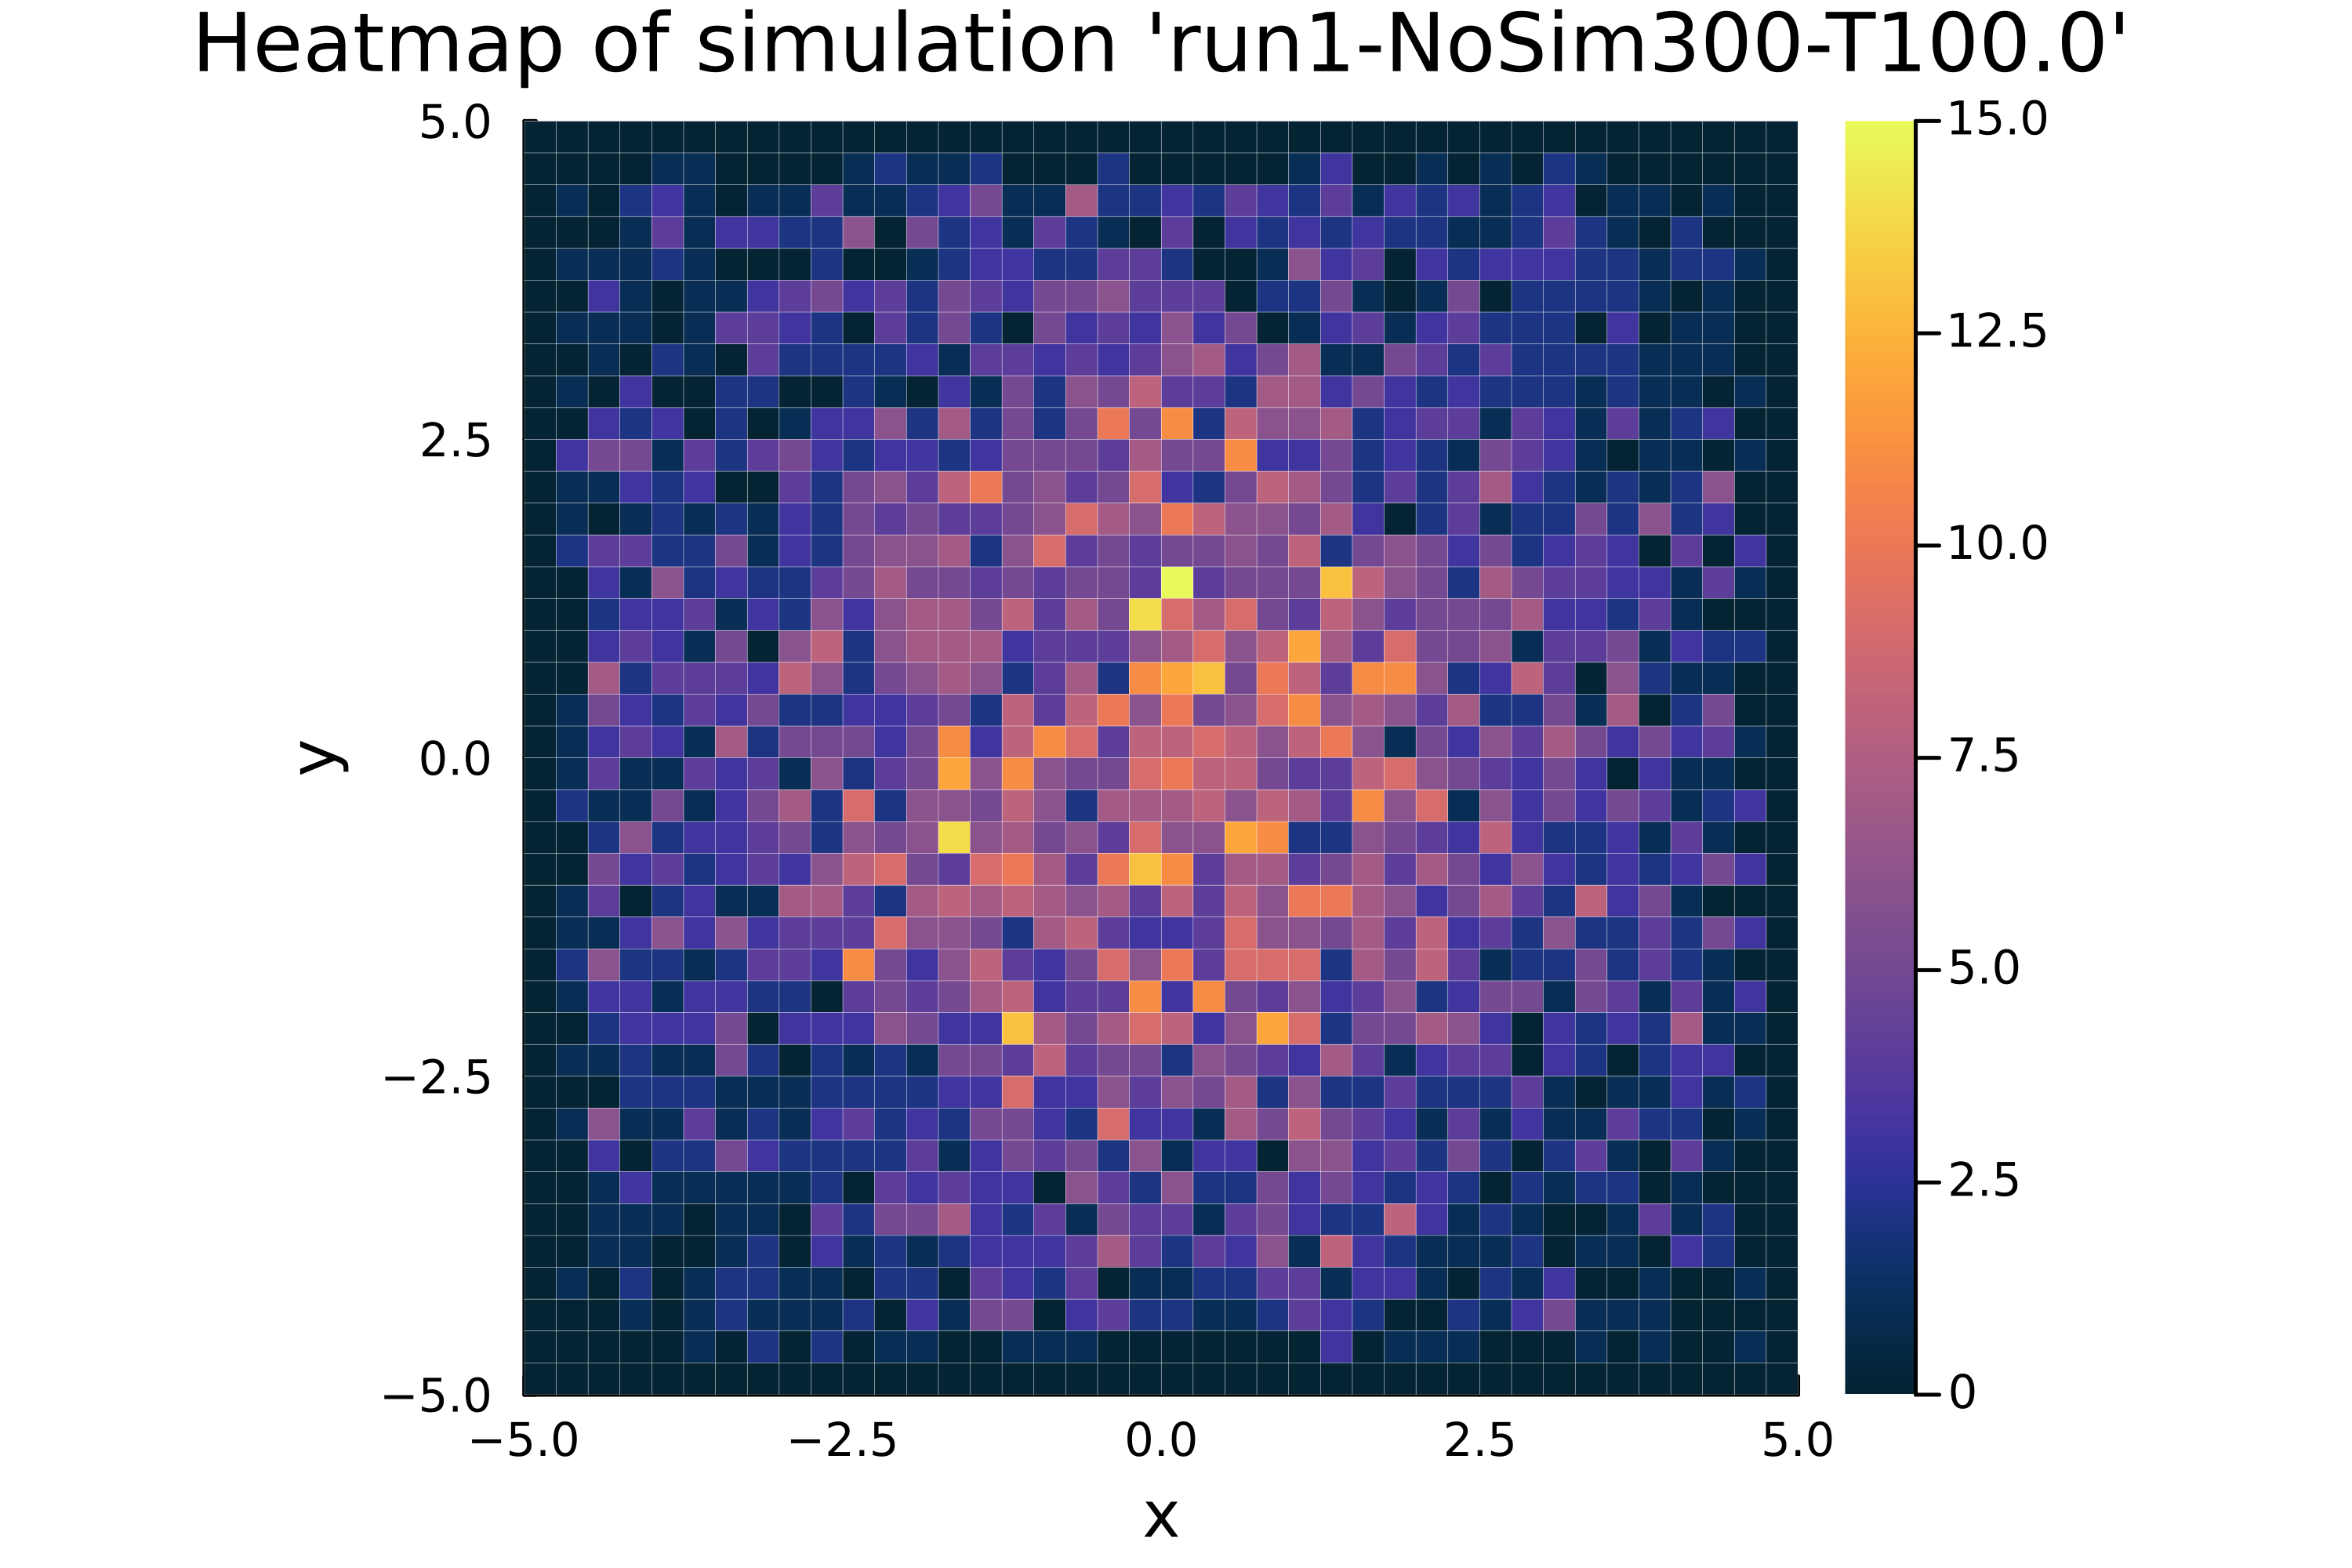
\includegraphics[width=\textwidth]{sanity-check/Heatmap-run1-NoSim300-T100.0/heatmaps/heatmap-run1-NoSim300-T100.0-sampleTime25000.png}
	\end{subfigure}
	\label{fig:model_illus}
\end{figure}


\newpage
\subsection*{Second big simulation}
Here is our most recent simulation parameters:
\begin{itemize}
    \item 100 cells are spawned normally distributed at the domain but without overlaps  
    \item 20 wall points per cell 
    \item Diffusitivity constant $D=100.0$
    \item bachelor scalings, but wihtout interior angle force for better stability
    \item $time interval = (0.0, 0.05)$
    \item $time step size = 10^{-4} = 0.0001$
    \item used radius billiard overlap 
    \item 3 simulations ran 
    \item $grid = [-5,5]^2$ with discretisation step size $\delta x = 0.25$
\end{itemize}

% FIGURE OF SECOND BIG SIMULATION
\begin{figure}[h!]
	\centering
	\begin{subfigure}{0.4\textwidth}
		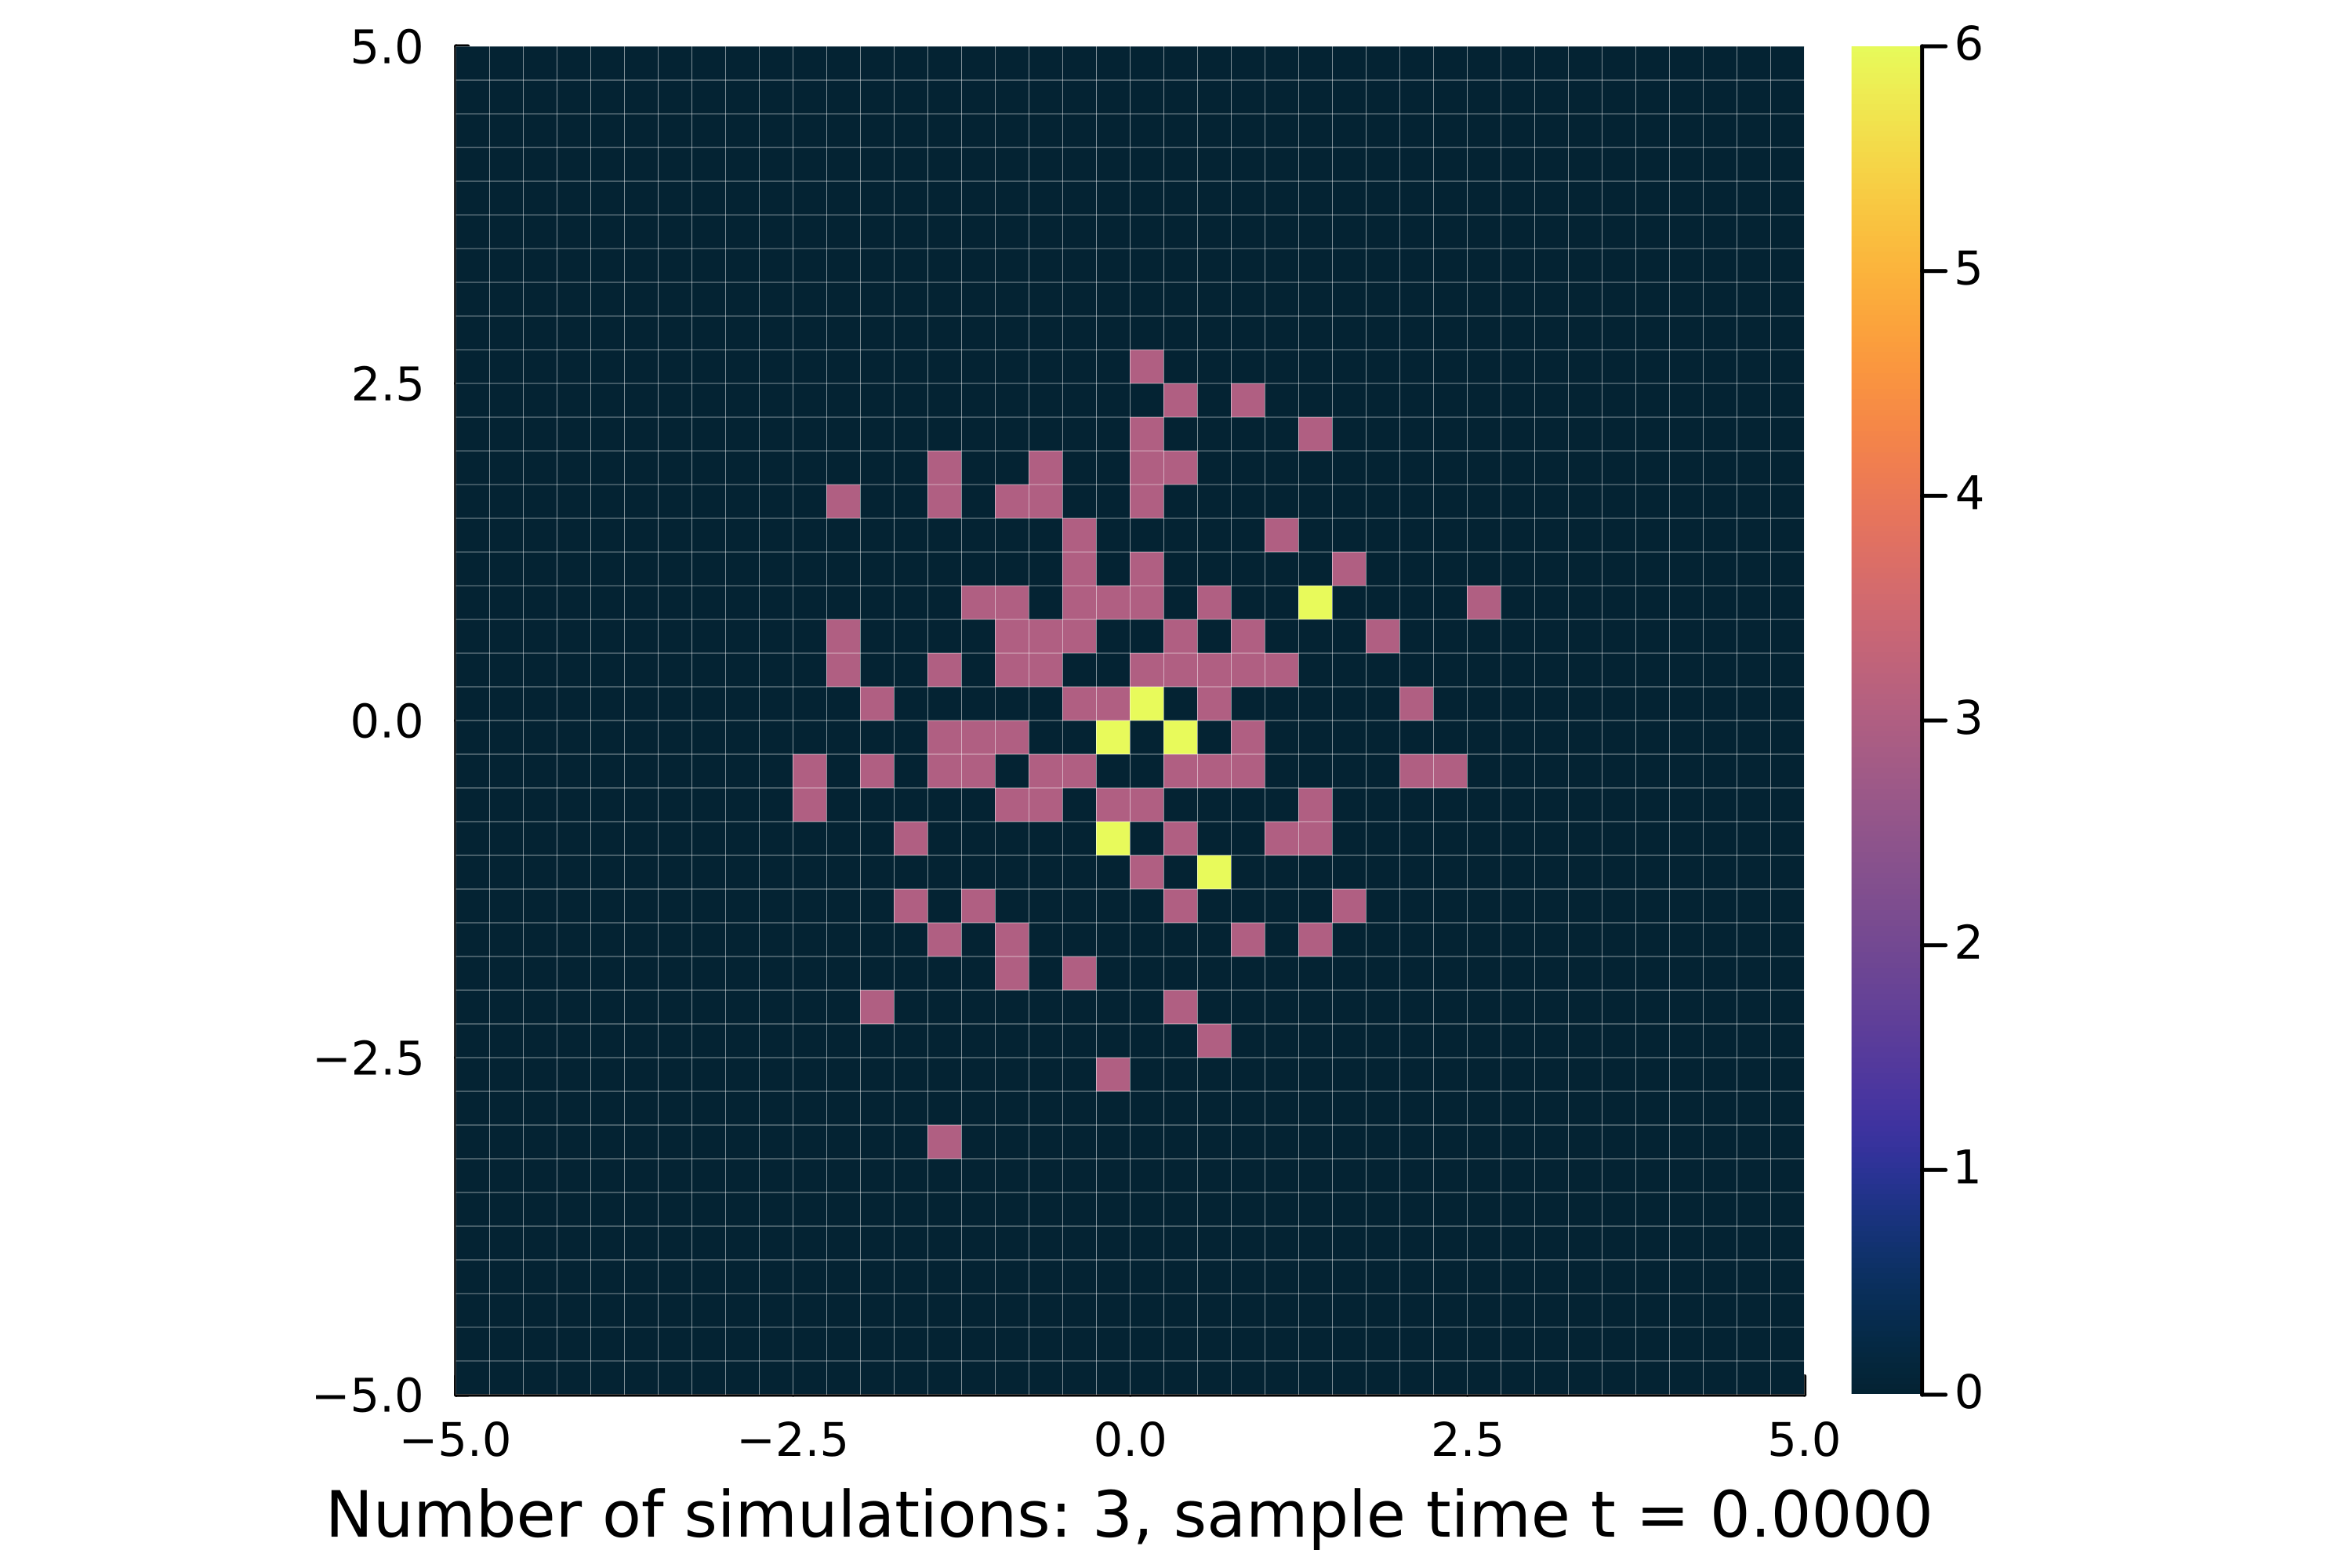
\includegraphics[width=\textwidth]{sanity-check/imitate-hardsphere-bruna-test1/heatmaps/heatmap-imitate-hardsphere-bruna-test1-sampleTime0.0.png}
	\end{subfigure}
	\hfill
	\begin{subfigure}{0.4\textwidth}
		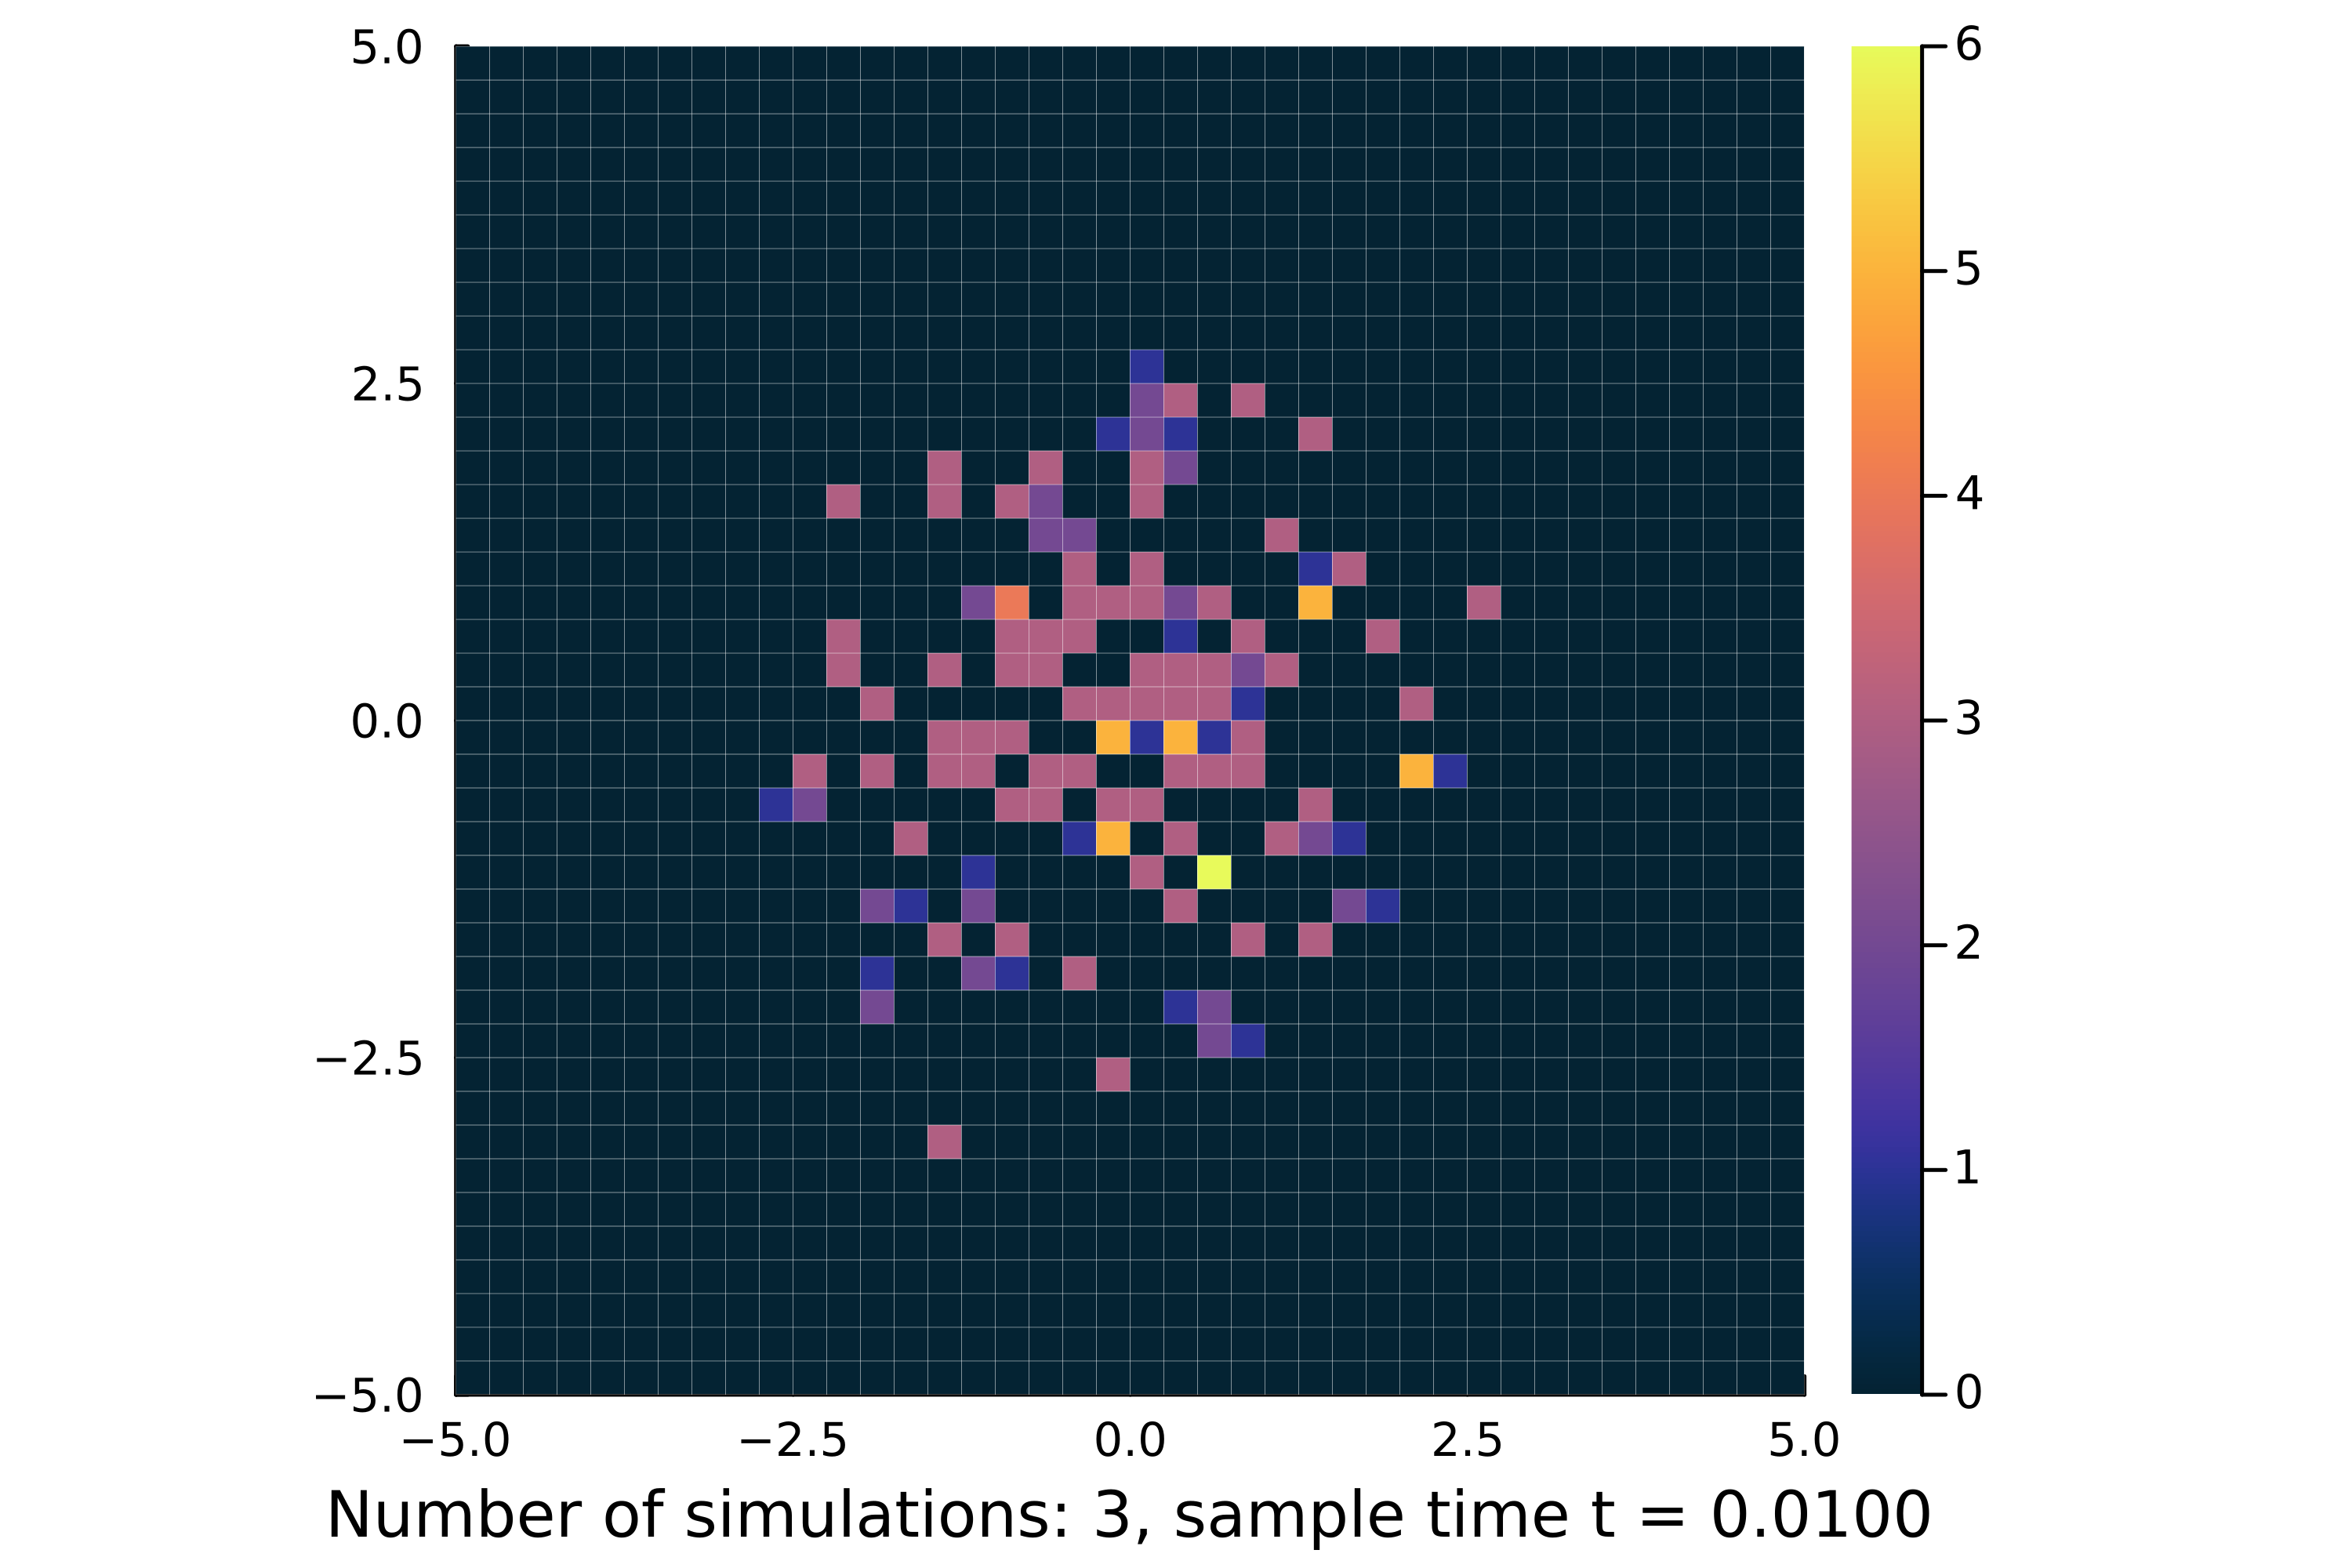
\includegraphics[width=\textwidth]{sanity-check/imitate-hardsphere-bruna-test1/heatmaps/heatmap-imitate-hardsphere-bruna-test1-sampleTime0.01.png}
	\end{subfigure}
	\hfill
	\begin{subfigure}{0.4\textwidth}
		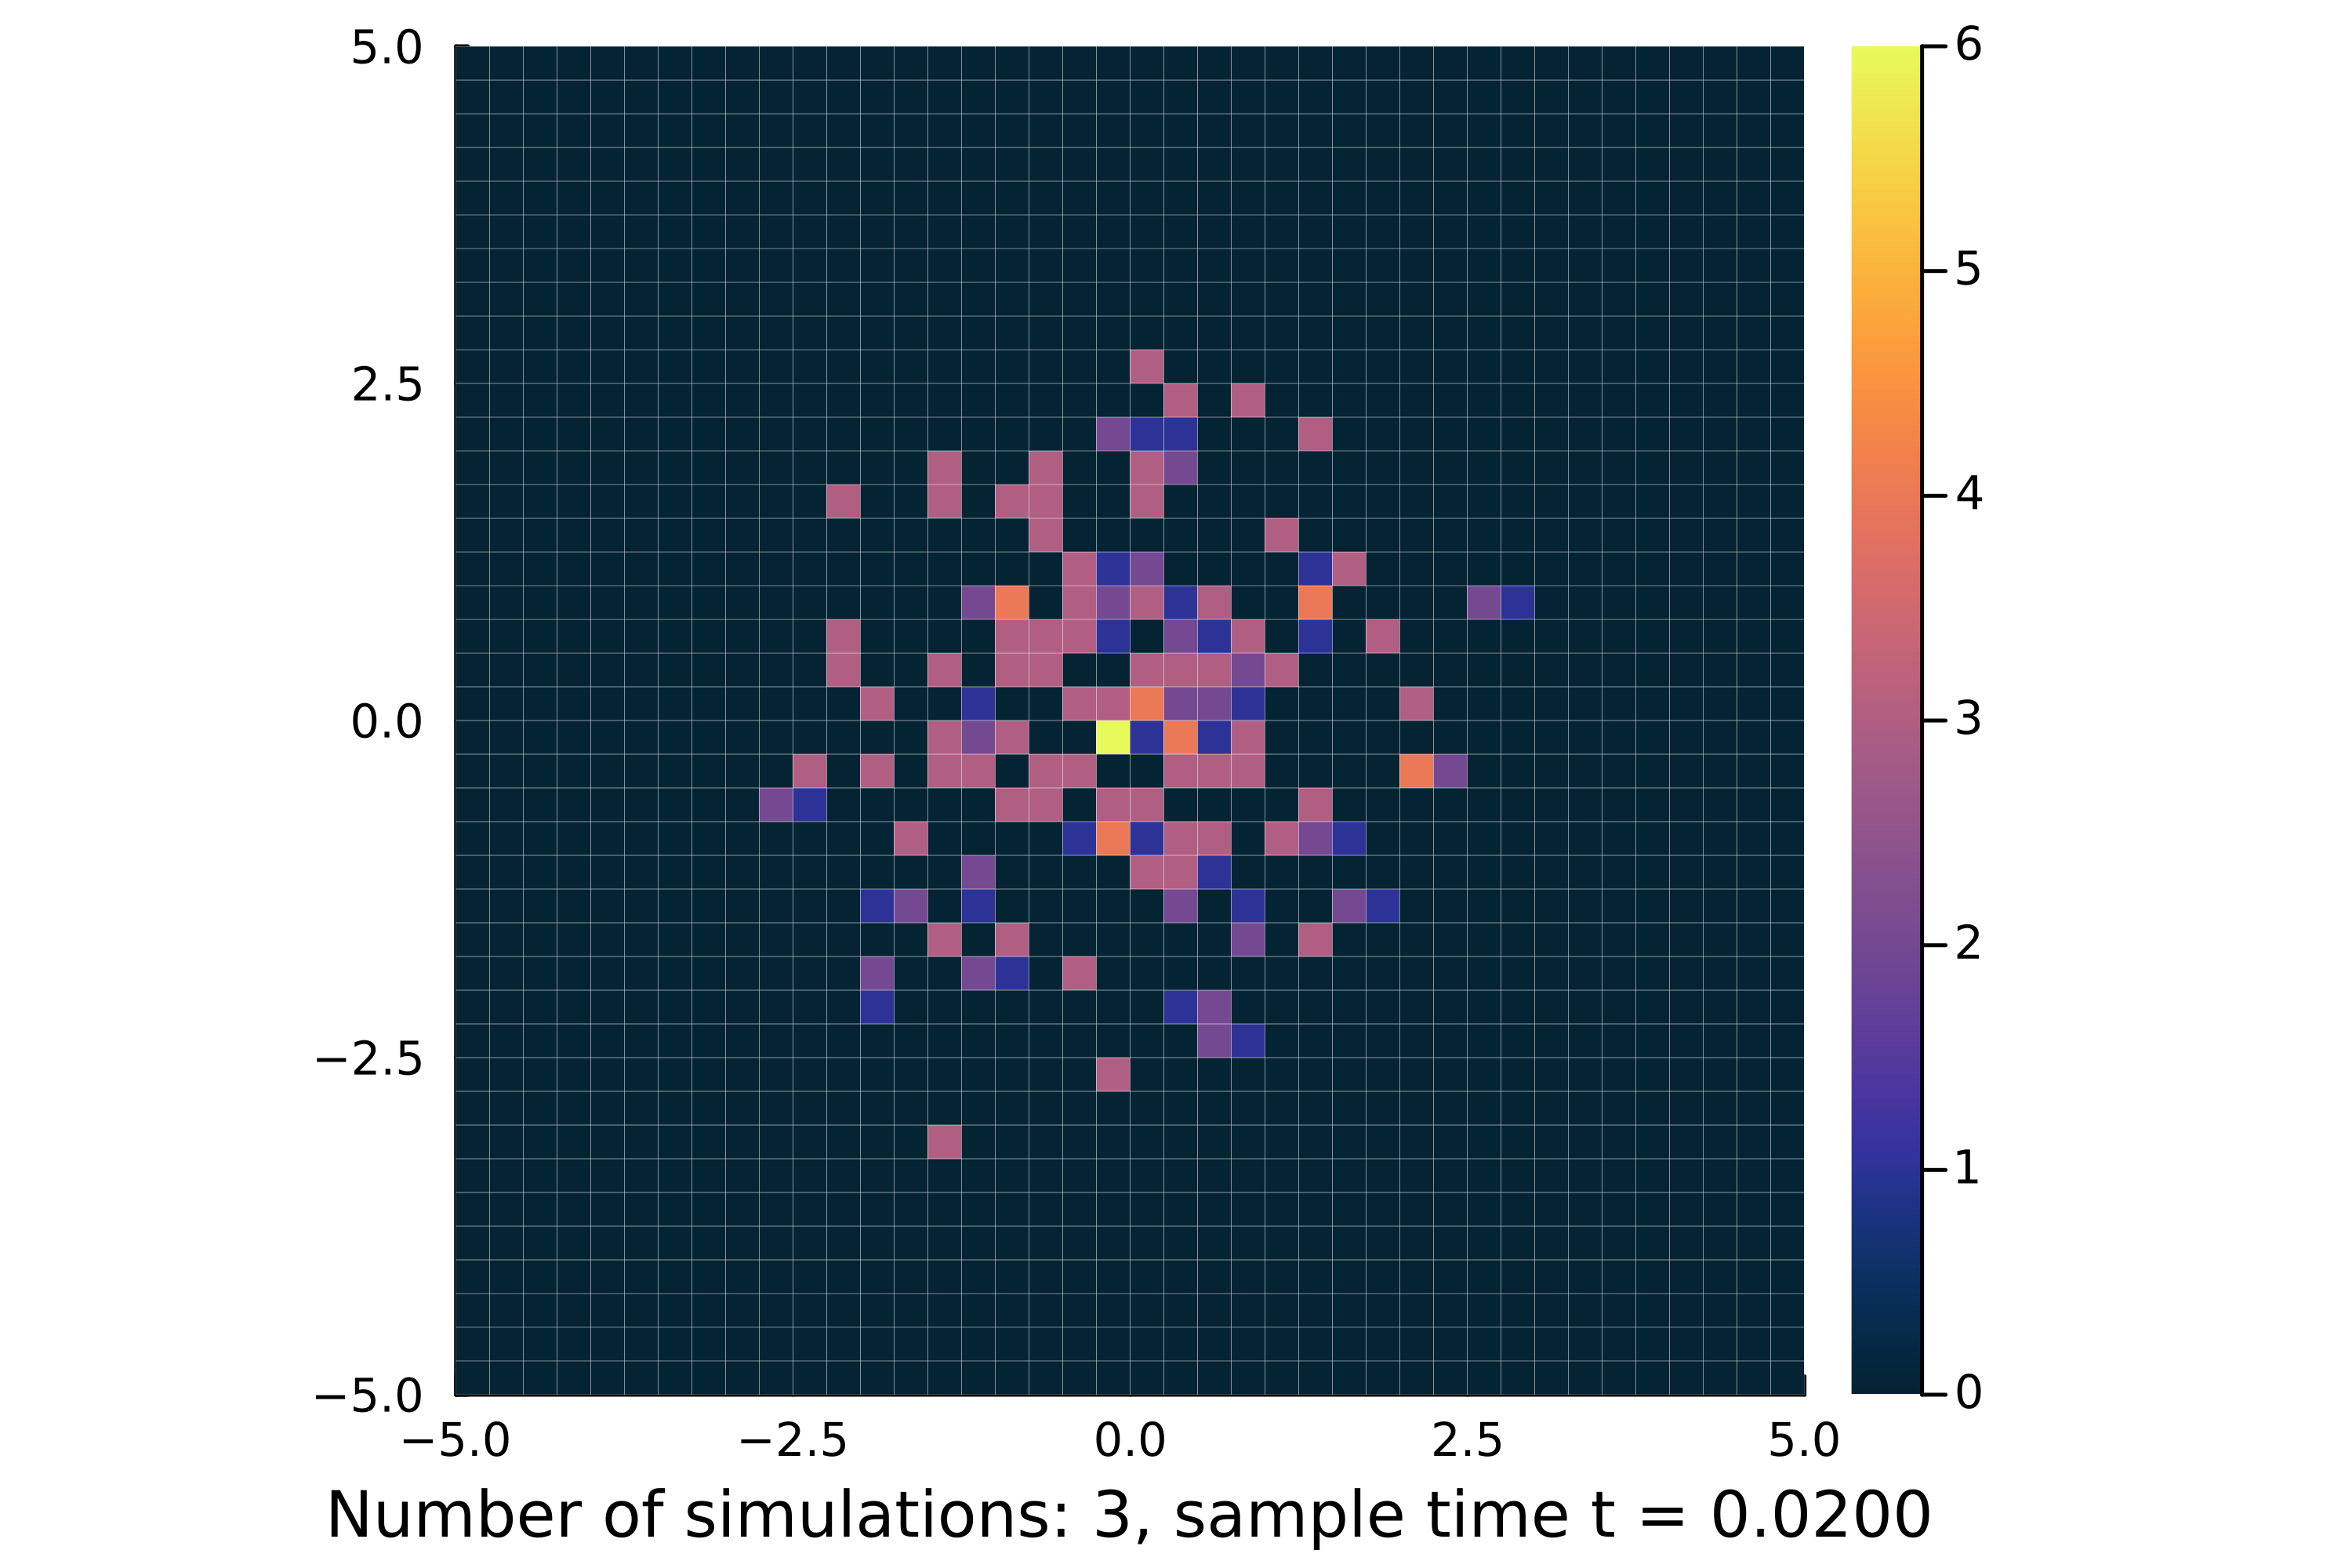
\includegraphics[width=\textwidth]{sanity-check/imitate-hardsphere-bruna-test1/heatmaps/heatmap-imitate-hardsphere-bruna-test1-sampleTime0.02.png}
	\end{subfigure}\hfill
	\begin{subfigure}{0.4\textwidth}
		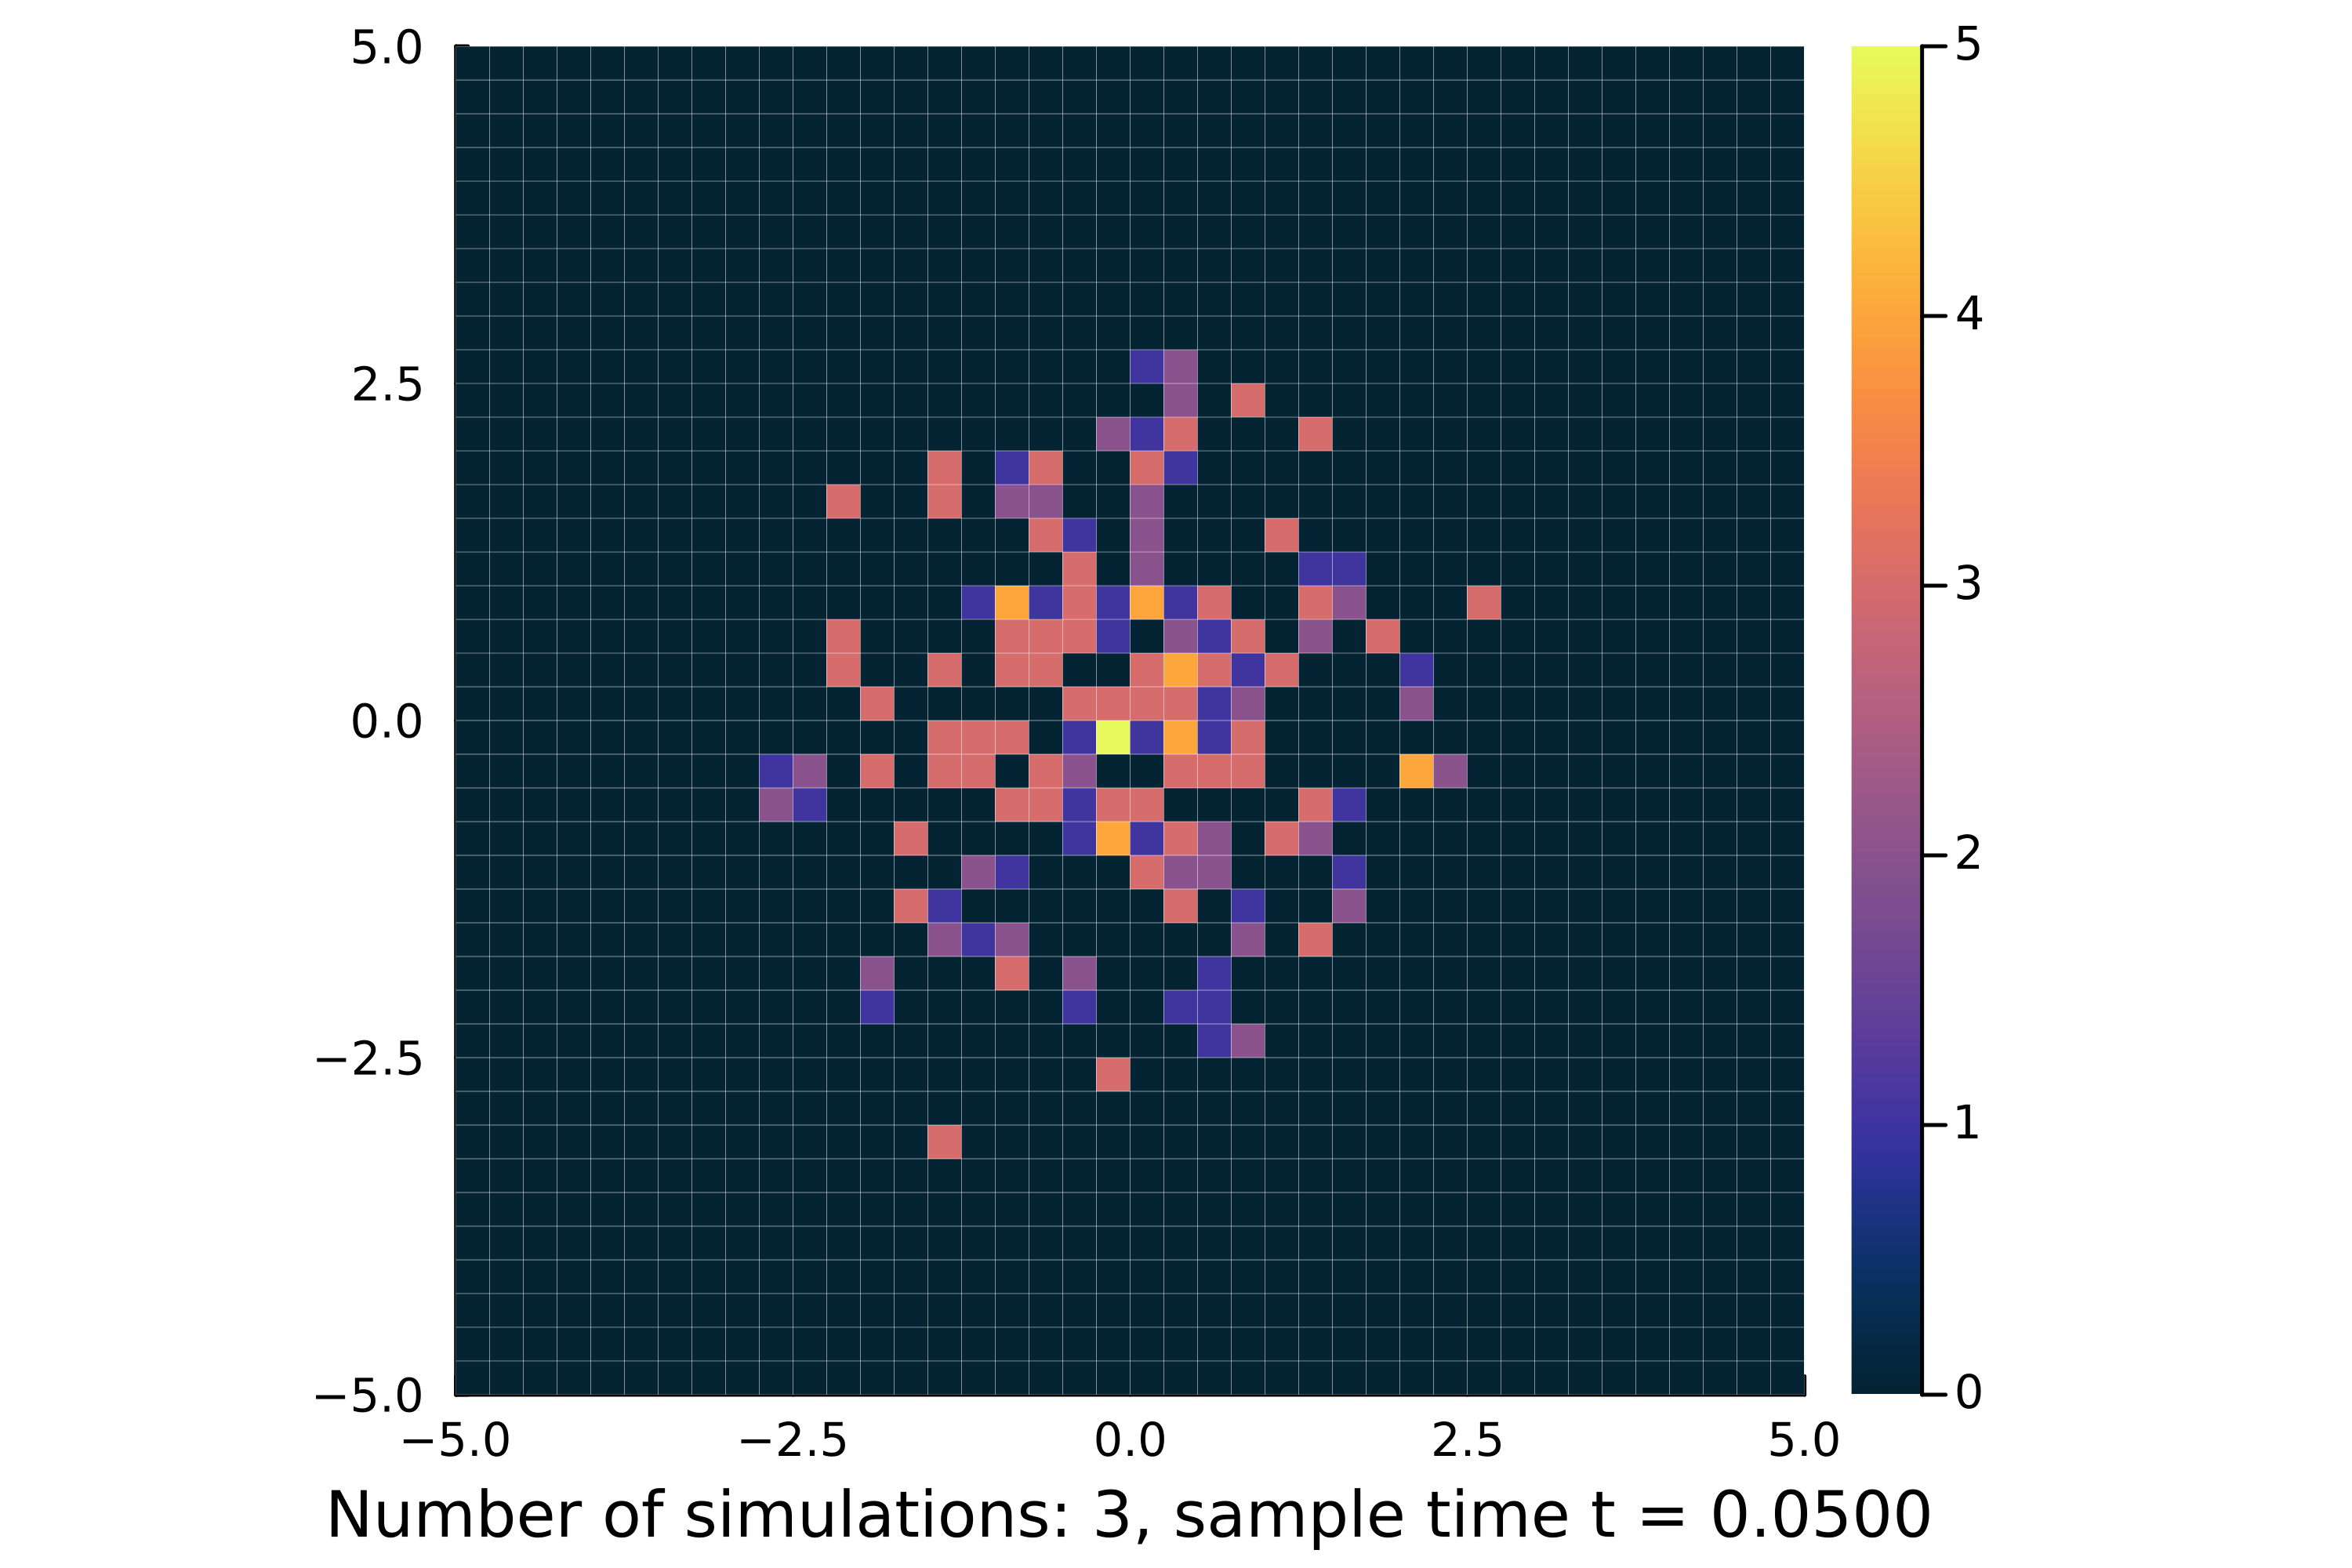
\includegraphics[width=\textwidth]{sanity-check/imitate-hardsphere-bruna-test1/heatmaps/heatmap-imitate-hardsphere-bruna-test1-sampleTime0.05.png}
	\end{subfigure}
	\label{fig:model_illus}
\end{figure}

\newpage
\subsection*{Overlaps}
\textbf{bachelor overlap (l 441 in energies.jl)}
\textbf{billiard overlap (l 474 in energies.jl)}
\textbf{combination of first 2 overlap  (l 539 in energies.jl)}
\textbf{radiusOverlapForceCells overlap (l 506 in energies.jl)}

\newpage
\subsection*{Next Steps}
\begin{itemize}
	\item Recreate chapman12 heatmap 
	
	\item 
	$
	initial condition: X' = \sqrt{10} X + 1, \quad \text{where } X \sim N(0,1) \\
	NoCells' = x (NoCells = 400) \\
	radius' = y (radius = 0.005) \\
	$AND ALSO$ radius' = 0 $ and without interaction [other parameters the same?] $
	time = [0.00,0.05], \delta t = 10^{-5} \\
	NoSimulations = 10^4 \\
	$Maybe run on linux work station in Z21$
	$
	\item parallelize code 
	\item use same color grading as in chapman12 (name?)

\end{itemize} 


